% This is "sig-alternate.tex" V2.1 April 2013
% This file should be compiled with V2.5 of "sig-alternate.cls" May 2012
%
% This example file demonstrates the use of the 'sig-alternate.cls'
% V2.5 LaTeX2e document class file. It is for those submitting
% articles to ACM Conference Proceedings WHO DO NOT WISH TO
% STRICTLY ADHERE TO THE SIGS (PUBS-BOARD-ENDORSED) STYLE.
% The 'sig-alternate.cls' file will produce a similar-looking,
% albeit, 'tighter' paper resulting in, invariably, fewer pages.
%
% ----------------------------------------------------------------------------------------------------------------
% This .tex file (and associated .cls V2.5) produces:
%       1) The Permission Statement
%       2) The Conference (location) Info information
%       3) The Copyright Line with ACM data
%       4) NO page numbers
%
% as against the acm_proc_article-sp.cls file which
% DOES NOT produce 1) thru' 3) above.
%
% Using 'sig-alternate.cls' you have control, however, from within
% the source .tex file, over both the CopyrightYear
% (defaulted to 200X) and the ACM Copyright Data
% (defaulted to X-XXXXX-XX-X/XX/XX).
% e.g.
% \CopyrightYear{2007} will cause 2007 to appear in the copyright line.
% \crdata{0-12345-67-8/90/12} will cause 0-12345-67-8/90/12 to appear in the copyright line.
%
% ---------------------------------------------------------------------------------------------------------------
% This .tex source is an example which *does* use
% the .bib file (from which the .bbl file % is produced).
% REMEMBER HOWEVER: After having produced the .bbl file,
% and prior to final submission, you *NEED* to 'insert'
% your .bbl file into your source .tex file so as to provide
% ONE 'self-contained' source file.
%
% ================= IF YOU HAVE QUESTIONS =======================
% Questions regarding the SIGS styles, SIGS policies and
% procedures, Conferences etc. should be sent to
% Adrienne Griscti (griscti@acm.org)
%
% Technical questions _only_ to
% Gerald Murray (murray@hq.acm.org)
% ===============================================================
%
% For tracking purposes - this is V2.0 - May 2012

\documentclass{sig-alternate-05-2015}
\usepackage[utf8]{inputenc}

\begin{document}

% Copyright
\setcopyright{acmcopyright}
%\setcopyright{acmlicensed}
%\setcopyright{rightsretained}
%\setcopyright{usgov}
%\setcopyright{usgovmixed}
%\setcopyright{cagov}
%\setcopyright{cagovmixed}


% DOI
\doi{10.475/123_4}

% ISBN
\isbn{123-4567-24-567/08/06}

%Conference
\conferenceinfo{AsianPLoP 2016}{February 24-26, Taiwan.}

%\acmPrice{\$15.00}

%
% --- Author Metadata here ---
\conferenceinfo{WOODSTOCK}{'97 El Paso, Texas USA}
%\CopyrightYear{2007} % Allows default copyright year (20XX) to be over-ridden - IF NEED BE.
%\crdata{0-12345-67-8/90/01}  % Allows default copyright data (0-89791-88-6/97/05) to be over-ridden - IF NEED BE.
% --- End of Author Metadata ---

\title{A Misuse Pattern for the Web Browser: Modification of traffic}
%\subtitle{[Extended Abstract]
%\titlenote{A full version of this paper is available as
%\textit{Author's Guide to Preparing ACM SIG Proceedings Using
%\LaTeX$2_\epsilon$\ and BibTeX} at


\numberofauthors{3} %  in this sample file, there are a *total*
% of EIGHT authors. SIX appear on the 'first-page' (for formatting
% reasons) and the remaining two appear in the \additionalauthors section.
%

\author{
\alignauthor
Paulina Silva\\
  \affaddr{Departamento de Informática}\\
  \affaddr{Universidad Técnica Federico Santa María}\\
  \affaddr{Valparaíso, Chile}\\
  \email{pasilva@alumnos.inf.utfsm.cl}
% 2nd. author
\alignauthor
Raúl Monge\\
  \affaddr{Departamento de Informática}\\
  \affaddr{Universidad Técnica Federico Santa María}\\
  \affaddr{Valparaíso, Chile}\\
  \email{rmonge@inf.utfsm.cl}
% 3rd. author
\alignauthor 
Eduardo B. Fernandez\\
  \affaddr{Department of Computer \(\&\) Electrical Engineering and Computer Science}\\
  \affaddr{Florida Atlantic University}\\
  \affaddr{Florida, USA}\\
  \email{ed@cse.fau.edu}
}

\maketitle
\begin{abstract}
Currently a lot of software developments create systems that are connected to the Internet, which allows to add functionality within a system and facilities to their \textit{Stakeholders}. This leads to depend in a \textit{web client}, as the \textit{Web Browser}, which allows access to services, data or operations that the system delivers. Nevertheless, the Internet influences the attack surface of the new system, and unfortunately many stakeholders and developers are not aware of the risks they are exposed. The lack of Security Education in Software developers of a project, the low and scattered documentation of each browser (and standardization), could become a great flaw in big architectural developments which depends on the browser to do their services. We are studying some security attacks in the web browser by describing them in the form of misuse patterns. A misuse pattern describes how an information misuse is performed from the point of view of the attacker. It defines the environment where the attack is performed, how the attack is performed, countermeasures to stop it, and how to find forensic information to trace the attack once it happens. We are building a catalog of misuse patterns and we present here one we called: Modification of traffic in the Web Browser. A catalog of misuse patterns will help designers to evaluate their designs with respect to possible threats.
\end{abstract}


%
% The code below should be generated by the tool at
% http://dl.acm.org/ccs.cfm
% Please copy and paste the code instead of the example below. 
%
\begin{CCSXML}
<ccs2012>
 <concept>
  <concept_id>10010520.10010553.10010562</concept_id>
  <concept_desc>Computer systems organization~Embedded systems</concept_desc>
  <concept_significance>500</concept_significance>
 </concept>
 <concept>
  <concept_id>10010520.10010575.10010755</concept_id>
  <concept_desc>Computer systems organization~Redundancy</concept_desc>
  <concept_significance>300</concept_significance>
 </concept>
 <concept>
  <concept_id>10010520.10010553.10010554</concept_id>
  <concept_desc>Computer systems organization~Robotics</concept_desc>
  <concept_significance>100</concept_significance>
 </concept>
 <concept>
  <concept_id>10003033.10003083.10003095</concept_id>
  <concept_desc>Networks~Network reliability</concept_desc>
  <concept_significance>100</concept_significance>
 </concept>
</ccs2012>  
\end{CCSXML}

\ccsdesc[500]{Computer systems organization~Embedded systems}
\ccsdesc[300]{Computer systems organization~Redundancy}
\ccsdesc{Computer systems organization~Robotics}
\ccsdesc[100]{Networks~Network reliability}




\keywords{Web Browser, Web Client, Modular Architecture, Browser Architecture, Reference Architecture, Browser Infrastructure Pattern}

\section*{Introduction}
%hablar sobre ataques de ingeniería social


\section{Patrón de Mal Uso: Modificación de tráfico en el \textit{Web Browser}}
En esta sección presentaremos un patrones de mal uso que describe la amenaza encontrada en el patrón Browser Infrastructure que hemos obtenido en este trabajo.
Una de las amenazas es que un atacante haya sido capaz de comprometer la respuesta obtenida desde el Provider contactado. El atacante podría tratar de reemplazar algunos parámetros de la respuesta del provider, entregando al Browser User un contenido distinto al original.

\subsection{Intent}
Un atacante podría cambiar contenido o dar uno diferente al esperado cuando el \textit{Web Browser} (Browser User) recibe la response del Servidor o Provider. Realizando esta acción, el navegador podría interpretar la información de una manera distinta a que si hubiera recibido el tráfico original.

\subsection{Contexto}
Un navegador web obtiene resources desde un Provider para poder satisfacer un Browser User que lo necesita. Un Provider posee resources en forma de páginas web, servicios web u otro tipo. El Provider generalmente consiste en una Web App o Web server, que puede permitir entrada y salida de datos a otras aplicaciones, normalmente éstos están construidos usando HTML, Javascript y CCS. Sea que éste desea entregar servicios, como también otros deseen conectarse a él, todo tipo de comunicación estará encima del protocolo HTTP. Un Provider, dependiendo del tipo, puede llegar a recibir muchas peticiones de diversos Host para obtener recursos de éste. Dependiendo del tipo de peticiones, éstas pueden o no ser permitidas. Aquellas que son permitidas, el Provider generará una response a la \textit{request} del Host, la cuál terminará llegando de vuelta (o no) al Browser Client que generó el \textit{request}.

\subsection{Problema}
¿Cómo podría un atacante engañar al Browser User y Host, por medio de la modificación de tráfico entre las entidades participantes en la comunicación? Es posible que un atacante esté escondido entre medio de la comunicación que hay entre el Host y el Provider, lo que resulta en que el contenido modificado podría afectar dentro del Web Content Renderer o el Browser Client. Esto en consecuencia podría traer diferentes resultados, desde el robo de información privada del Browser User que utiliza el Browser Client para personalizar la navegación como también los token de autenticación hacia los Providers que el Browser User ha utilizado previamente. Dependiendo del tipo de atacante, es posible que éste pueda incluso afectar al Host del \textit{Browser}, dejando que el atacante pueda realizar actos maliciosos con los recursos del Host. 
El ataque puede sacar ventaja de las siguientes vulnerabilidades:
\begin{itemize}
  \item El \textbf{origen} u \textbf{origin} que define el Same Origin Policy que hace cumplir el \textit{Browser} difiere en cada tipo de \textit{Web Browser} \cite{W3C-SOP,Reis2009, Jackson2008, Crowley2010, Paola2006}.
  \item El \textbf{origin} no es suficiente como método de aislación entre resources (páginas web, scripts, css y otros) \cite{Silic2010, Barth2009, Yason, Liu2012}.
  \item Cualquiera puede crear una extensión o plugin, etc. para algún tipo de \textit{Browser} y hacerlo pasar como algo inofensivo, pero el usuario no se daría cuenta que un ataque Man-in-the-Browser podría estar ocurriendo \cite{Dougan2012,Utakrit2009,Liu2012,Barth2010}.  Éste programa, posiblemente malicioso, podría afectar el tráfico sin que queden rastros, pues tiene permisos del usuario al ser éste mismo quien autorizó su instalación.
  \item Es posible afectar al Browser Client, y en consecuencia al Host, sin tener que buscar vulnerabilidades en el \textit{Web Browser}. Solamente utilizando métodos de ingeniería social, sobre el usuario del Host basta para lograr un ataque, pues es \textbf{el eslabón más débil}.
  \item La arquitectura para extender la funcionalidad del navegador, a través de extensiones, plugins y otros, depende demasiado del manufacturador. Y probablemente posee una gran superficie de ataque.
\end{itemize}

El ataque puede ser facilitado por:
\begin{itemize}
  \item Existen muchas herramientas para realizar ataques de ingeniería social, lo que permite hacer que el Browser User acepte realizar la instalación de extensiones o plugin maliciosos más fácilmente.
  \item Cualquier script basado en texto puede ser usado para explotar el intérprete del navegador web. Muchas veces también es posible utilizar los mismos elementos del lenguaje de scripting para poder pasar ciertas barreras de seguridad entregadas por el SOP, pues el lenguaje está basado en prototipos. 
  \item Los manufacturadores de Navegadores no poseen aún mecanismos de defensa que permitan identificar efectivamente cuando un recurso puede ser malicioso.
  \item Los métodos de cifrado no pueden hacer nada contra un ataque que puede modificar el tráfico antes de enviar o después de recibir el mensaje.
  \item No existen mecanismos de defensa estandarizados, pues cada manufacturador realiza lo necesario para la marca a la que se acopla. Si el Host posee muchos browser, la superficie de ataque es bastante mayor.
\end{itemize}
\subsection{Solución - Estructura}
La solución estructural usada es la misma creada por el patrón Browser Infrastructure que se revisó en el capítulo 4. La clase Attacker es cualquier entidad que podría llevar a cabo una acción arriesgada contra la integridad del \textit{Browser}, usuario, Host y Provider (Figura \ref{fig:BIMisuse}). El atacante es capaz tanto de interceptar las response que el Provider envía al Browser Client usando al Host como receptor, o haciendo que el \textit{Browser} realice modificaciones en el input que va hacia el Provider, utilizando scripts u otro resources.

\begin{figure*}[h!t]
  \centering
  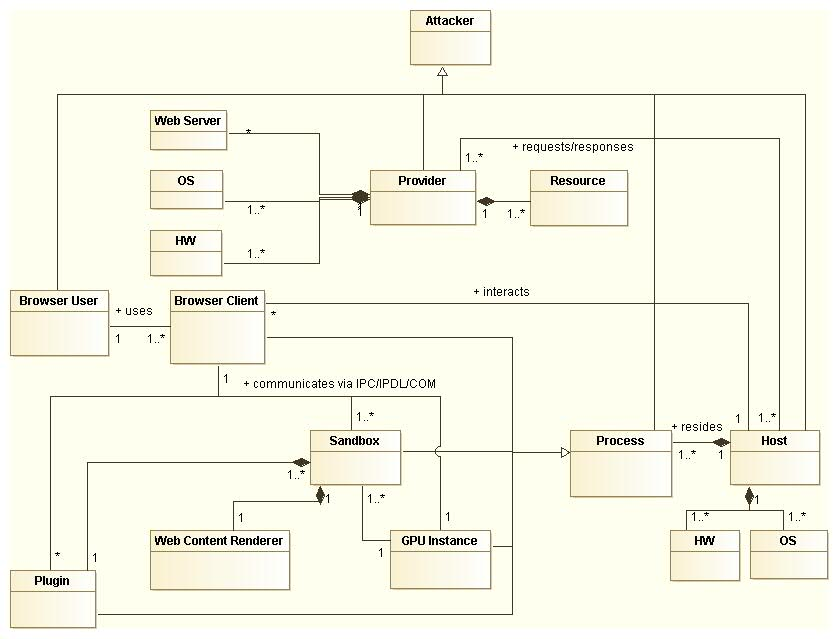
\includegraphics[scale=0.55]{figures/patronMisuse_v2.jpg}
  \caption{Diagrama de Clases para el patrón de Misuse.}
  \label{fig:BIMisuse}
\end{figure*}

\subsection{Dinámica}
En la figura \ref{fig:SeqMisuse} se muestra la serie de pasos necesarios, para realizar uno de los tantos mal usos que se pueden realizar durante el caso de uso Realizar \textit{request}. El atacante queda entre el Browser Client y el Host, interceptando la realización del \textit{request} original y modificando el tráfico a su gusto; usualmente un ataque basado en este mal uso se le llama Man-in-the-Browser (MITB) \cite{Liu2012, Barth2010, Utakrit2009, Dougan2012}. Esto podría perfectamente suceder cuando el Browser User ha permitido la instalación de plugins, extensiones o programas externos en el Host y Browser Client.

\begin{figure*}[h!t]
  \centering
  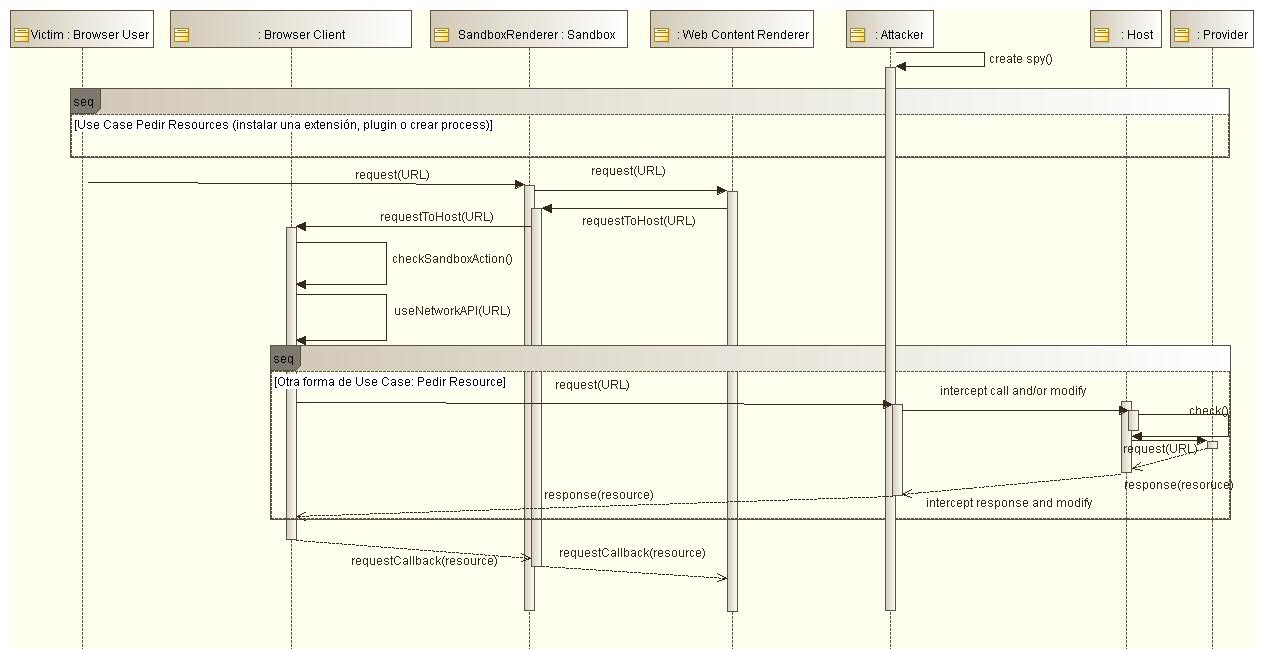
\includegraphics[scale=0.52]{figures/patronMisuseSeq_v2.jpg}
  \caption{Diagrama de Secuencia para el Mal uso: Modificación de tráfico en el \textit{Web Browser}.}
  \label{fig:SeqMisuse}
\end{figure*}

  
  \subsubsection{Sumario} El atacante intercepta el tráfico entre Host y Browser Client.
  \subsubsection{Actor} Atacante
  \subsubsection{Precondiciones} Para que el ataque pueda pasar desapercibido, es necesario que el Browser User o el usuario detrás del browser haya caído primero en un ataque de ingeniería social o el atacante haya podido instalar directamente un proceso o componente malicioso en el Host directamente.
  \subsubsection{Descripción}
      \begin{enumerate}
        \item Un atacante utiliza alguna técnica de ingeniería social o vulnerabilidad en el sistema, para crear una entidad que se encargará de estar entre medio del Browser Client y el Provider. Para esto realiza el caso de uso \textbf{Pedir Resources} para que el proceso, plugin o extensión se aloje en el Host.
        \item Un Browser User desea hacer un \textit{request} a cierta URL, por lo que los primeros pasos de \textbf{Realizar Request} son similares.
        \item En el momento en que el Browser Client va a realizar la llamada al sistema para enviar el mensaje del Host al Provider, el Browser Client llamará al plugin, extensión o process malicioso, pues el Browser Client ha sido intervenido para que realice esa acción de este modo.
        \item El atacante entonces recibirá todo el tráfico del Browser Client, el cuál podría modificar a su antojo.
        \item Finalmente la víctima está totalmente comprometida.
      \end{enumerate}
  \subsubsection{Post condiciones} La víctima quedará completamente comprometida y probablemente no sea posible detectar la alteración del mensaje, pues también es posible que se modifiquen los log del Host.
  \subsubsection{Usos Conocidos} El \textit{Web Browser} es un software que posee diversas implementaciones, por lo tanto la cantidad de vectores de ataque es significativa. Algunos de éstos son:
      \begin{itemize}
        \item  Una extensión basada en la arquitectura de Chrome o la API WebExtension Firefox, podría interceptar los datos antes que llegue al Browser Client \cite{Paola2006} o dado a una vulnerabilidad del mismo elemento un atacante se está aprovechando de su funcionalidad para realizar ataques \cite{Liu2012, Barth2010}. Dado que el Plugin, la extensión o el process son elementos que el Host confía, es posible que el ataque sea indetectable y los métodos de cifrado no sirven como medida de mitigación.
        \item Éste tipo de ataque puede ser usado como base para otros ataques más avanzados. Un ejemplo es cuando el \textit{Browser} posee vulnerabilidades \textit{cross-origin javascript capability leaks}, donde los diferentes modelos de seguridad usados por Javascript y el DOM pueden interferir entre sí, causando que una petición \textit{cross-origin} se pueda realizar aún cuando SOP debería ser capaz de detener tal ataque \cite{Barth2009}.
      \end{itemize}


\subsection{Consecuencias}
  El mal uso tiene las siguientes consecuencias para el Attacker:
  \begin{itemize}
    \item Objetivos: pueden ser diversos, destacándose el vandalismo, personificar a otra persona u obtener una ganancia monetaria. Mientras el atacante se pueda interponer entre el Host y el tráfico que se envía al Provider, la confidencialidad e integridad de los datos está completamente perdida. La privacidad del usuario ya no se puede asegurar tampoco.
    \item Silencioso: Dado que el atacante ha logrado interponerse entre las llamadas de sistema que se realizan al Host para enviar los datos al Provider, el Host no reconocerá ni logueará ninguna anomalía. Las llamadas hechas al Host son totalmente legales y nada fuera de lo normal para éste.
    \item El atacante podría realizar acciones que afecten la integridad del Host.
  \end{itemize}
  Posibles fuentes de fallo:
  \begin{itemize}
    \item Si el Browser User es capaz de evitar o ignorar el ataque de Ingeniería Social realizado al comienzo, no existiría este mal uso. Esto debe considerar que el usuario también no se encuentre con páginas o contenido malicioso, que podrían afectar otro componente de \textit{Browser}, pero que causarían en el mismo efecto del Mal Uso señalado.
  \end{itemize}

\subsection{Contramedidas} 
  Para prevenir este tipo de mal uso se recomienda tomar las siguientes medidas preventivas:
  \begin{itemize}
    \item Servicios de Reputación como Smart Screen de Internet Explorer y Download Application de Google Chrome, ayudan a identificar páginas y contenido/resources que podrían contener malware que se instale como plugins, entensiones o process en el Host del Browser User.
    \item Entregando educación sobre los peligros de navegar por Internet y aclarar al usuario que él es la última línea de defensa contra éste tipo de ataques.
    \item White y Black list instaladas en los browser son una medida preventiva para evitar la navegación en páginas o recursos maliciosos ya conocidos.
    \item Navegadores como Google Chrome e Internet Explorer ofrecen el Sandboxing. Éste mecanismo de defensa limita las acciones del atacante, que pudieran afectar la integridad del sistema.
  \end{itemize}

\subsection{Evidencia Forense}
  ¿Dónde es posible encontrar evidencia?
  Dependiendo de lo deseado por el atacante, las acciones que cometerá pueden diferir. Sin embargo el log interno del browser debería de poder servir para auditar el sistema, esto gracias a que mientras no se haya encontrado una vulnerabilidad en el Sandbox del \textit{Browser}, el atacante no puede borrar completamente sus huellas.

\subsection{Patrones relacionados}
  \begin{itemize}
    \item En el patrón Browser Infrastructure, el Browser Client actúa como el Reference Monitor explicado en \cite{fernandez2001pattern}.
  \end{itemize}


\section*{Conclusions}
%A Web browser appears to be a medium complexity software for users and developers without security experience, but unfortunately this piece of software allows a variaty of attack vectors, to the user using it as well the system with which interacts. Therefore it is important to understand its structure and how it interacts with internal or/and external Stakeholders.

%It is expected that in the future most \textit{Web Browser} will take the form of a Modular Architecture. Therefore, it is important that developers know the internal processes of \textit {browser} when developing a system that will interact with it. The Reference Architecture prepresented here, it is aimed at providing the basic knowledge of the components and interactions between \textit{Web Browser} and external Provider for resources; as well as the threats that exist within it.

%A part of our Reference Architecture has been built through the abstraction of found documentation, through the Browser Infrastructure pattern. We created our first architectural pattern for the infrastructure of \textit{Web Browser}; to help others to understand holistically the components, interactions and relationships of this system. Furthermore it has been possible to characterize the Stakeholders and one of the most important use case. From what we have known, this is the second Reference Architecture for the \textit{Browser} built.

%The proposed work allows a better understanding of this system called Web Browser by using our partially Reference Architecture, this is also helpful to understand existing threats. Furthermore, as it is not subject to specific implementations, it is possible to generalize certain results in other browsers.


We have presented some web browser threats as a form of misuse patterns which describe in a systematic way how one misuses is performed.
El objetivo de éste capítulo es conocer y visualizar los mal usos del sistema, en este caso del Browser, para poder educar a los desarrolladores de proyectos que basan sus sistemas en el uso de éste. A través del listado de amenazas es posible detectar o inferir actividades de mal uso que pueden aparecer en uno o más casos de uso, que podrían resultar en una vulneración del sistema.

iniciar un pequeño catálogo de Patrones de Mal Uso. Esto permitirá condensar el conocimiento obtenido en el punto anterior a través de documentos semi-formales, lo que permitirá generar una guía para comunicar los conceptos relevantes que pudieran afectar la relación existente entre un desarrollo de software y el navegador.

Un catálogo de Misuse Patterns podría ser de gran valor en el Desarrollo de Sistemas que interactúan con el navegador, pues provee a desarrolladores un medio para evaluar los diseños de sus sistemas, al analizar las posibles amenazas del Browser que pudieran afectar al software que está siendo construido.



\section*{Future Work}
Future work will be related to the creation of a Security Reference Architecture for the \textit{Web Browser} using the same methodology presented here. Other patterns related to Browser Infrastructure pattern will be obtained in order to complete the AR already begun, such as the Web Content Renderer pattern and Browser Kernel. An example of the type of work to be carried out can be seen in \cite{fernandez2014security} where this study carries out activities to build secure software and evaluate the safety levels of a system already built.

We plan to build more Misuse patterns, for the Browser Infrastructure pattern, to continue the study of the possible threats in the \textit{Browser}, as a way to educate Developers and Stakeholders. While at the same time these patterns will allow the construction of the Security Reference Architecture. In the same line, in addition to finding potential threats existing in the system, we need to find countermeasures or security defenses to prevent or foresee such threats through security patterns on the reference architecture built. This is possible to perform under the same exercise already conducted in this work, looking for threats at each action for each use case of the Browser.

As for \textit{Web Browsers}, attacks based on social engineering does not seem to decrease at any good time, because there is no current technology that can detect a \(100 \% \) without no false positives the potential threats they can bring. Technologies such as CAMP (Content-Agnostic Malware Protection) appear to be part of the solution, but are still far from perfect.


\bibliography{refTodas}  
\bibliographystyle{IEEEtran}


\end{document}
